%%%%%%%%%%%%%%%%%%%%%%%%%%%%%%%%%%%%%%%%%
% University Assignment Title Page 
% LaTeX Template
% Version 1.0 (27/12/12)
%
% This template has been downloaded from:
% http://www.LaTeXTemplates.com
%
% Original author:
% WikiBooks (http://en.wikibooks.org/wiki/LaTeX/Title_Creation)
%
% License:
% CC BY-NC-SA 3.0 (http://creativecommons.org/licenses/by-nc-sa/3.0/)
% 
% Instructions for using this template:
% This title page is capable of being compiled as is. This is not useful for 
% including it in another document. To do this, you have two options: 
%
% 1) Copy/paste everything between \begin{document} and \end{document} 
% starting at \begin{titlepage} and paste this into another LaTeX file where you 
% want your title page.
% OR
% 2) Remove everything outside the \begin{titlepage} and \end{titlepage} and 
% move this file to the same directory as the LaTeX file you wish to add it to. 
% Then add \input{./title_page_1.tex} to your LaTeX file where you want your
% title page.
%
%%%%%%%%%%%%%%%%%%%%%%%%%%%%%%%%%%%%%%%%%
%\title{Title page with logo}
%----------------------------------------------------------------------------------------
%	PACKAGES AND OTHER DOCUMENT CONFIGURATIONS
%----------------------------------------------------------------------------------------

\documentclass[12pt]{article}
\usepackage[english]{babel}
\usepackage[utf8x]{inputenc}
\usepackage{amsmath}
\usepackage{amsfonts}
\usepackage{mathtools}
\usepackage{enumerate}% http://ctan.org/pkg/enumerate
\DeclarePairedDelimiter{\ceil}{\lceil}{\rceil}
\usepackage{dsfont}
\usepackage{float}
\usepackage{graphicx}

% Pour faire des coeurs, trèfles, carreaux, etc.
\DeclareSymbolFont{extraup}{U}{zavm}{m}{n}
\DeclareMathSymbol{\varheart}{\mathalpha}{extraup}{86}
\DeclareMathSymbol{\vardiamond}{\mathalpha}{extraup}{87}

\usepackage{hyperref}
\hypersetup{
    colorlinks,
    citecolor=black,
    filecolor=black,
    linkcolor=black,
    urlcolor=black
}
\usepackage[colorinlistoftodos]{todonotes}
\usepackage[
top    = 3cm,
bottom = 4cm,
left   = 3cm,
right  = 3cm]{geometry}
\begin{document}

\begin{titlepage}

\newcommand{\HRule}{\rule{\linewidth}{0.5mm}} % Defines a new command for the horizontal lines, change thickness here

\center % Center everything on the page
 
%----------------------------------------------------------------------------------
%	HEADING SECTIONS
%----------------------------------------------------------------------------------

\textsc{\Large Oral exam INFO-F-408}\\[0.5cm] % Major heading such as course name
\textsc{\large Computability \& complexity}\\[0.5cm] % Minor heading such as course title

%----------------------------------------------------------------------------------
%	TITLE SECTION
%----------------------------------------------------------------------------------
\HRule \\[0.4cm]
{ \huge \bfseries Exam's questions}\\[0.4cm] % Title of your document
\HRule \\[1.5cm]
 
%----------------------------------------------------------------------------------
%	AUTHOR SECTION
%----------------------------------------------------------------------------------
% If you don't want a supervisor, uncomment the two lines below and remove the section above
Mourad \textsc{Akandouch}\\[0cm] % Your name
Daoud  \textsc{YEMNI    }\\[0cm] % Your name
       \textsc{         }\\[2cm] % Your name
%----------------------------------------------------------------------------------
%	DATE SECTION
%----------------------------------------------------------------------------------
{\large \today}\\[3cm] % Date, change the \today to a set date if you want to be precise

%----------------------------------------------------------------------------------
%	LOGO SECTION
%----------------------------------------------------------------------------------

\includegraphics[width=0.4\textwidth]{logo.jpg}\\[1cm] % Include a department/university logo - this will require the graphicx package
%----------------------------------------------------------------------------------
\end{titlepage}

\tableofcontents
\newpage
\section{Summary and checklist}
\paragraph{}


\section{Introduction}
\subsection{What is the relation between decision problems and languages ?}
\paragraph{}
\underline{Réponse de Daoud}
\paragraph{}
Un problème décisionnel est un problème auquel la réponse aux instances est soit oui, soit non. Un langage décisionnel est un langage auquel chaque instance de ce langage peut être reconnu (ou décidé) par une machine de Turing. Une instance d'un problème peut être transformer en un ensemble de mots tel que :
\begin{itemize}
\item L'ensemble des mots représentant les instances positives du problème
\item L'ensemble des mots représentant les instances négatives du problème
\end{itemize} 
De ce fait, nous pouvons transformer l'ensemble des mots en un langage qui pourra être reconnu (ou décidé) par une machine afin de résoudre le problème.

\paragraph{}
(Note : En toute logique, nous récupérerons que les ensembles de mots/langage des instances posivites d'un problème)

\paragraph{}
(\#Daoud, je ne sais pas si c'est très clair)
\paragraph{}
\underline{Réponse de Mounir}
\paragraph{}
Un problème est dit de décision si la réponse aux instances du problème est soit oui soit non.
\paragraph{}
Exemples :
\begin{itemize}
\item Déterminer si oui ou non un nombre entier n est pair est un problème de décision
\item Par contre déterminer la longueur minimale du circuit qui passe par tous les sommets d’un graphe n’est pas un problème de décision.
\end{itemize}
\paragraph{}
Un problème de décision constitue un langage. En effet, un problème possède plusieurs instances qui sont encodés par des mots définis sur un alphabet $\Sigma$. L’ensemble de tous les mots définis sur $\Sigma$ peut être partitionné en deux sous-ensembles :
\begin{itemize}
\item Les mots représentant des instances du problème pour lesquelles la réponse est oui, nous appellerons ces instances les instances positives du problème
\item Les mots représentant des instances du problème pour lesquelles la réponse est non, ces sont les instances négatives
\end{itemize}
\paragraph{}
Un problème de décision peut donc être caractérise par l’ensemble des mots qui sont des instances positives du problème. Un ensemble de mots définis sur le même alphabet est un langage.
\paragraph{}
Résoudre un problème de décision équivaut à reconnaitre le langage des encodages des instances positives du problème.
\subsection{Define finite automata and explain the difference between deterministic and nondeterministic finite automata. (cf. Sections 1.1 and 1.2)}
\paragraph{}
Un automate fini est défini comme 5-uple $(Q, \Sigma, \delta, q_{0}, F)$ où :
\begin{enumerate}
\item $Q$ est l'ensemble fini des états possibles
\item $\Sigma$ est un alphabet, il s'agit de l'ensemble fini des symboles acceptés par l'automate. 
\item $\delta$ est défini différemment selon qu'on soit un automate déterministe ou pas. Dans le cas d'un automate déterministe, $\delta$ est une fonction dite "de transition" définie comme suit : $\delta : Q \times \Sigma \rightarrow Q$. C'est-à-dire une fonction qui reçoit en argument un état et un symbole, et retourne l'état atteint.
\paragraph{}
Dans le cas d'un automate non-déterministe, il y a une petite différence au niveau de la fonction de transition. Elle est définie comme suit. $\delta : Q \times \Sigma_{\epsilon} \rightarrow \mathcal{P}(Q)$ où $\Sigma_{\epsilon}$ est aussi l'alphabet auquel on rajoute le symbole vide $\epsilon$. Ici, la fonction reçoit un état et un symbole en argument et retourne \textbf{un ensemble d'états atteignables}. $\mathcal{P}(Q)$ est une notation qui signifie \textit{"l'ensemble de tous les sous-ensembles de Q"}.
\paragraph{Exemple} 
\begin{itemize}
\item $\delta(q_{3}, z) = q_{5}$ signifie que lorsqu'on est à l'état $q_{3}$ et qu'on lit le symbole $z$, alors on atteint l'état $q_{5}$. Ici, la transition est déterministe.
\item  $\delta(q_{15}, \alpha) = \{q_{1}, q_{2}, q_{51}\}$ signifie que l'orsqu'on est à l'état $q_{15}$ et qu'on lit le symbole $\alpha$, nous pouvons atteindre les états $q_{1}$, $q_{2}$ et $q_{51}$. La transition, ici, est non-déterministe. 
\end{itemize}

\item $q_{0}$ est l'état à partir duquel l'automate démarre. On l'appelle l'état initial.
\item $F$ représente l'ensemble des états qui acceptent.
\end{enumerate}

\paragraph{}
Une autre différence réside également dans la manière dont ces automates sont exécutés. Dans le cas d'un déterministe, l'exécution est déterminé. D'un état, en lisant un symbole, nous atteignons\textbf{ au maximum 1} état. Tandis que dans le non-déterministe, lorsque plusieurs états sont atteignables depuis un état, l'automate va \textbf{se cloner et atteindre tous les états} (comme un fork() ). Évidemment, en faisant cela, certains clones n'atteindront pas un état d'acceptance. Donc, dès lors qu'un automate non-déterministe ne peut plus avancer (il lit un symbole où aucun état n'est atteignable), le clone se tue. Un automate non-déterministe accepte \textbf{si au moins une exécution accepte} (c'est-à-dire qu'il y a \textbf{au moins une suite de transition qui mène à un état d'acceptance}).
\begin{figure}[H]
\centering
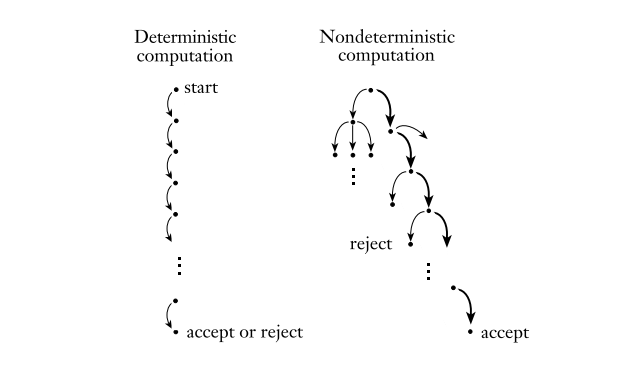
\includegraphics[width=\textwidth]{img_2_2__0}
\caption{Deterministic and nondeterministic computations with an accepting branch}
\end{figure}

\section{Computability (chapters 3-4-5)}
\subsection{What is a Turing Machine ?}
\paragraph{}
La machine de Turing est très similaire aux automates finis mais avec une mémoire infinie et non-restreinte. Il s'agit d'un modèle beaucoup plus précis de ce que sait faire un vrai ordinateur. Toutefois, même une machine de Turing ne peut pas résoudre tous les problèmes.
\paragraph{}
La machine de Turing utilise un ruban infini comme mémoire. Sa tête de lecture/écriture \textbf{peut bouger vers la gauche ou vers la droite} et peut \textbf{lire et écrire sur le ruban}.
\paragraph{}
Initiallement, la machine possède uniquement l'input dans son ruban et est vide partout ailleurs. Si la machine a besoin de stocker de l'information, elle peut écrire ces informations sur le ruban. Pour lire les informations qui ont été écrites sur le ruban, la machine peut bouger sa tête de lecture/écriture vers l'endroit où est stocké cette information dans le ruban. La machine continue de s'exécuter jusqu'à ce qu'elle décide de produire une sortie \textit{accept} ou \textit{reject}. 

\paragraph{}
Si la machine n'atteint pas un de ces deux états, elle s'exécutera pour toujours, sans jamais s'arrêter. Donc, contrairement aux automates fini, ici, la machine s'arrête \textbf{dès qu'elle} atteint un état d'acceptance ou de rejet. Dans le cas d'un automate, l'arrêt ne s'occure pas dès que l'un de ces états est atteint.
\paragraph{}
Formellement, une machine de Turing est définie comme un 7-uple ($Q$, $\Sigma$, $\Gamma$, $\delta$, $q_{0}$, $q_{accept}$, $q_{reject}$) où $Q$, $\Sigma$ et $\Gamma$ sont des ensembles finis et:
\begin{enumerate}
\item $Q$ est l'ensemble des états
\item $\Sigma$ est l'alphabet sans le symbole vide.
\item $\Gamma$ est l'alphabet \textbf{du ruban} où le symbole vide est compris dedans et $\Sigma \subseteq \Gamma$, c'est-à-dire que l'alphabet est un sous-ensemble de $\Gamma$.
\item $\delta : Q \times \Gamma \rightarrow Q \times \Gamma \times \{L, R\}$ est la fonction de transition. Elle prend en argument un état et un symbole du ruban, et retourne l'état atteignable correspondant, le symbole à écrire et la direction vers laquelle la tête de lecture/écriture va bouger. $L$ signifie $left$ (gauche) et $R$ signifie $right$ (droite).
\paragraph{Exemple} $\delta(q, a) = (r, b, L)$ signifie que lorsqu'on est dans l'état $q$ et qu'on lit le symbole $a$ sur le ruban, alors on atteint l'état r, on remplace le symbole $a$ par $b$ et on bouge la tête de lecture/écriture d'une case vers la gauche.
\item $q_{0}$ est l'état initial 
\item $q_{accept}$ est l'état d'acceptance 
\item $q_{reject}$ est l'état de rejet.
\end{enumerate}

\paragraph{}
Initiallement, une machine de Turing $M$ démarre tel que suit : $M$ reçoit son input $w = w_{1}...w_{n} \in \Sigma^{*}$ sur les cases les plus à gauches du ruban, le reste du ruban est rempli de symbole vide. La tête de lecture/écriture démarre sur la première case (la plus à gauche) du ruban.Si $M$ tente de bouger à gauche malgré qu'il soit déjà sur la case la plus à gauche, la tête ne bouge pas. Le premier symbole blanc, puisque n'apparaîssant pas dans $\Sigma$, correspond à la fin de l'input.

\paragraph{}
Lorsqu'une machine de Turing s'exécute, des changements se font dans l'état courant, le contenu courant du ruban et la position actuelle de la tête de lecture/écriture. L'association de ces trois éléments est appelé \textbf{une configuration} de la machine de Turing. Une configuration est représenté d'une manière assez spéciale. Considérons que nous sommes dans l'état $q$ et deux chaines de caractères $u$ et $v$ sur le ruban. On écrit $u$ $q$ $v$ pour dire que nous sommes à l'état $q$, le contenu actuel du ruban est $uv$ et que la tête de lecture/éctiture est située sur le premier symbole de $v$.
\paragraph{Exemple} $1011q_{7}01111$ signifie que nous sommmes dans une configuration tel que le contenu du ruban est 101101111, nous sommes dans l'état $q_{7}$ et la tête de lecture/écriture est situé sur le deuxième zéro.

\subsection{What is a Turing-recognizable language ? What is a Turing-decidable language ? Explain the difference between the two notions and why we use deciders to formalize the intuitive notion of algorithm.}
\paragraph{}
Un langage \textbf{Turing-reconnaissable} est un langage dont une machine de Turing reconnaît toutes les chaines de caractères. Si une machine de Turing 
ne reconnaît pas l'input, elle boucle éternellement.
\paragraph{}
Un langage \textbf{Turing-décidable} ou simplement \textbf{décidable} est un langage qu'une machine de Turing décide. C'est-à-dire que pour tout input sur le ruban, la machine décide de rejeter ou d'accepter. Elle ne bouclera jamais contrairement aux langages simplement reconnaissables.

\paragraph{}
Nous préférons utiliser des décideurs plutôt que des reconnaisseurs parce qu'avec un simple reconnaisseur, nous ne pouvons pas distinguer si un algorithme qui boucle éternellement ou s'il prend simplement beaucoup de temps à s'exécuter.

\subsection{Define the notion of multitape Turing Machine. Prove that every multitape Turing Machine has an equivalent single tape Turing Machine.}
\paragraph{}
Une machine de Turing multi-ruban est comme une machine de Turing ordinaire mais avec plusieurs ruban. Chacun de ces rubans possède sa propre tête de lecture/écriture. Initiallement, l'input apparaît sur le premier ruban et les autres sont vides. La fonction de transition est modifiée afin de permettre la lecture, l'écriture et le mouvement des têtes de lecture/écritures sur plusieurs ou tous les rubans simultanément. Formellement, la fonction est défini comme suit :
\begin{equation}
\delta : Q \times \Gamma^{k} \rightarrow Q \times \Gamma^{k} \times \{L, R, S\}^{k}
\end{equation}
où $k$ est le nombre de ruban.
\paragraph{Exemple} L'expression
\begin{equation}
\delta(q_{i}, a_{1}, ..., a_{k})  = (q_{j} , b_{1}, ..., b_{k}, L, R, ..., L)
\end{equation}
signifie que si nous sommes dans l'état $q_{i}$ et que les têtes de lecture/écriture des rubans 1 à $k$ lisent les symboles $a_{1}$ à $a_{k}$, alors la machine atteint l'état $q_{j}$, écrit les symboles $b_{1}$ à $b_{k}$ sur les rubans correspondant et bouge les têtes de lecture/écriture soit à gauche ($L$), soit à droite ($R$), soit reste sur place ($S$) sur les rubans correspondants.

\paragraph{Preuve que les multi-rubans ont un équivalent simple ruban}
Soit une machine de Turing multi-ruban $M$ et une autre mono-ruban $S$. Nous devons convertir $M$ en un équivalent mono-ruban.
L'idée principale est de montrer comment simuler $M$ avec $S$.

Disons que $M$ possède $k$ rubans. Alors $S$ simule l'effet de $k$ rubans en sauvegardant leur information sur un seul ruban. Pour ce faire, la machine utilise le nouveau symbole $\#$ comme délimiteur pour séparer les contenus de chaque ruban. En plus du contenu de ces rubans, $S$ doit garder une trace de la localisation des têtes. Elle le fait via l'alphabet du ruban (on rajoute des symboles). Un symbole avec un point au-dessus de celui-ci marque l'emplacement de la tête sur ce ruban. L'image suivante montre comment un mono-ruban peut représenter trois rubans.

\begin{figure}[H]
\centering
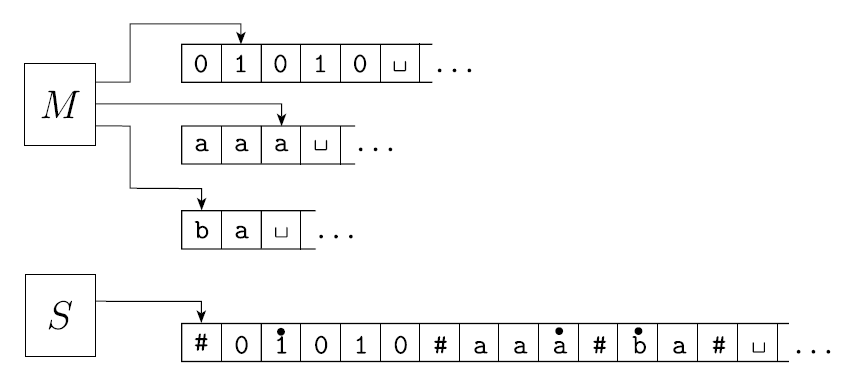
\includegraphics[width=\textwidth]{img_3_3__0}
\caption{Representing three tapes with one}
\end{figure}

\subsection{Prove that every nondeterministic Turing Machine has an equivalent deterministic Turing Machine.}

\paragraph{}
\textit{(Même comportement que la machine automate non-déterministe, la fonction de transition ne donne pas un résultat unique mais un ensemble de résultat)}

\paragraph{Preuve que toutes les TM non-déterministes ont un équivalent déterministe}

\paragraph{}
L'idée de la preuve est que nous pouvons simuler n'importe quel TM non-déterministe $N$ avec une déterministe que nous nommerons $D$. L'idée de la simulation est d'avoir $D$ qui teste toutes les branches possibles d'une exéctuion non-déterministe de $N$. Si $D$ accède à un état d'acceptance, $D$ accepte directement. 

\paragraph{}
Sinon, la simulation de $D$ ne terminera pas. Nous pouvons voir l'exécution de $N$ sur une entrée $w$ comme un arbre. Chaque branche de l'arbre représente une des branches créées par le non-déterminisme. Chaque noeud de l'arbre est une configuration $N$. La racine de l'arbre est la configuration au démarrage. $D$ 

\paragraph{}
$D$ va chercher dans l'arbre une configuration d'acceptance. Mener cette recherche soigneusement est cruciale pour que D ne visite pas l'arbre entier. Une idée tentante, mais mauvais, serait d'explorer l'arbre en profondeur (depth-first) parce que ce type de parcours va le plus profondément possible via une branche avant de pouvoir en explorer d'autres. 

\paragraph{}
Si $D$ devait explorer l'arbre de cette manière, $D$ pourrait descendre éternellement dans une branche qui se répète indéfiniment et ratera donc une configuration d'acceptance qui pourrait se trouver sur une autre branche. Du coup, il faut préférer une exploration en largeur (breadth-first). 

\paragraph{}
Cette stratégie explore toutes les branches de même profondeur avant d'explorer plus profondément. Cette méthode garantit que $D$ visitera chaque noeud de l'arbre jusqu'à rencontrer une configuration d'acceptance.

\paragraph{Preuve} La preuve utilise une TM à trois rubans. \textit{(et on sait que tous les multi-rubans possèdent un équivalent mono-ruban)}
La simulation de la TM déterministe $D$ possède trois rubans qui ont chacun une utilité particulière.
\begin{itemize}
\item Le premier ruban contiendra l'input originel et ne sera jamais altéré.
\item Le second ruban maintient une copie de la simulation non-déterministe de $N$ sur la branche qu'on parcourt actuellement.
\item Le troisième ruban garde une trace de la localisation
\end{itemize}

\begin{figure}[H]
\centering
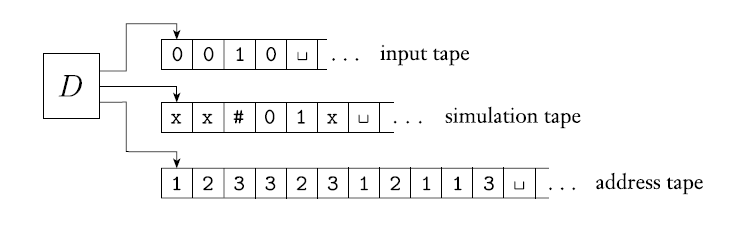
\includegraphics[width=\textwidth]{img_3_4__0}
\caption{Deterministic TM D simulating nondeterministic TM N}
\end{figure}
\paragraph{}
Parlons tout d'abord de la structure de donnée représentée dans le ruban 3. Chaque noeud dans l'arbre peut avoir au-plus $b$ fils où $b$ est la taille (le cardinal) du plus grand ensemble possible de choix en fonction de la fonction de transition de $N$.

\paragraph{}
À chaque noeud de l'arbre, nous assignons une adresse qui est une chaine de caractère de l'alphabet $\Gamma_{b} = \{1, 2, 3, ..., b\}$. 

\paragraph{Exemple} Nous assignons l'adresse $231$ au noeud que nous atteignons lorsque l'on part de la racine, suivi de son 2ème noeud, puis du 3ème noeud du 2ème noeud, et enfin, le premier noeud de ce troisième noeud qui lui-même est letroisième noeud d'un deuxième noeud qui, lui, est le deuxième noeud de la racine. Bref, cela représente le chemin de la racine jusqu'au dernier digit du nombre. Donc, racine $\rightarrow$ 2ème noeud $\rightarrow$ 3ème noeud $\rightarrow$ 1er noeud.
\paragraph{Algorithme}
\begin{enumerate}
\item Au départ, le ruban 1 contient l'input $w$, et les rubans 2 et 3 sont vides.
\item Copier le ruban 1 dans le ruban 2 et initialiser le ruban 3 à $\epsilon$.
\item Utiliser le ruban 2 pour simuler $N$ avec l'input $w$ sur une branche de ses exécutions non-déterministe. Avant chaque étape de $N$, consulter le symbole suivant sur le ruban 3 pour déterminer quel choix faut-il faire parmi ceux qui sont autorisés par la fonction de transition de $N$. S'il n'y a plus de symbole sur le ruban 3 ou si ce choix non-déterministe est invalide, annuler cette branche en allant à l'étape 4. Aussi, il faut aller à l'étape 4 si une configuration de rejet est rencontrée. Si une configuration d'acceptance est rencontrée, on accepte l'input.
\item Remplacer la chaine de caractère sur le ruban 3 par la chaine de caractère suivante dans l'ordre. Simuler la branche suivante de $N$ en allant à l'étape 2.
\end{enumerate}

\subsection{Explain what is an enumerator for a language. Prove that a language is Turing-recognizable if and only if it has an enumerator.}
\paragraph{}
Un énumérateur $E$ pour un langage est l'ensemble des chaines de caractères que cet énumérateur pourrait imprimer. Plus encore, $E$ peut générer les chaines de caractères du langage dans n'importe quel ordre, même avec répétitions.

\paragraph{Théorème} Un langage est TM-reconaissable si et seulement si un énumérateur l'énumère (le liste, le print...).
\paragraph{Preuve} Tout d'abord, montrons que si nous avons un énumerateur $E$ qui énumère un langage $A$, alors une machine de Turing $M$ reconnaît $A$. La machine de Turing $W$ travaille comme suit.

\paragraph{}
$M = $ "Sur l'input $w$ :
\begin{enumerate}
\item Exécuter $E$. À chaque fois que $E$ imprime une chaine de caractère, la comparer avec $w$.
\item Si $w$ apparaît dans la sortie de $E$, alors on \textit{accepte}."
\end{enumerate}

\paragraph{}
Clairement, $M$ accepte également les chaines de caractères qui apparaissent dans la liste de $E$.

\paragraph{}
Maintenant, faisons la procédure dans un autre sens. Si une machine de Turing $M$ reconnaît un langage $A$, nous pouvons construire l'énumérateur $E$ suivant pour $A$. Mettons que $s_{1}, s_{2}, s_{3}...$ soit une liste de toutes les chaînes de caractères dans $\Sigma^{*}$.

\paragraph{}
$E = $ "Ignore l'input.
\begin{enumerate}
\item Répéter ce qui suit pour $i = 1, 2, 3...$ :
\item Exécuter $M$ pour $i$ étapes sur chaque input $s_{1}, s_{2}...s_{i}$.
\item Si une des exécutions accepte, imprimer la chaine de caractère $s_{j}$ correspondante."
\end{enumerate}

\subsection{What is the Church-Turing thesis ? Give arguments in favor of it.}
\paragraph{}
\textit{"De manière informelle, cette thèse stipule que s’il existe un algorithme pour résoudre un problème, alors ce même problème peut être résolu à l’aide d’une machine de Turing.} 
\paragraph{}
\textit{Il convient cependant de souligner le fait qu’il ne s’agit là qu’une d’une thèse, et non pas d’un théorème. Il n’est en effet pas possible de démontrer ce théorème, puisqu’il n’existe aucune autre définition formelle à la notion d’algorithme. La thèse de Church-Turing définit donc un nouvel objet, les machines de Turing, pour caractériser une notion intuitive et ancienne
d’algorithme.}

\paragraph{}
\textit{Bien qu’il ne s’agisse là que d’une thèse, elle est largement admise et de nombreux arguments plaident en sa faveur :}
\begin{itemize}
\item \textit{De façon générale, personne n'a jamais pu exhiber une procédure de calcul réalisable par un esprit humain qu'une machine de Turing ne pourrait pas elle-même réaliser;}

\item \textit{Les machines de Turing peuvent subir des extensions (multi-ruban, non déterminisme...), mais aucune de ces extensions ne permet au modèle de reconnaitre d’avantage de langages. À chacune de ces extensions correspond une machine de Turing déterministe à ruban simple qui lui est équivalente ;}

\item \textit{De nombreux autres modèles de calcul ont été proposés pour caractériser la notion d’algorithme ($\lambda$-calcul, fonctions récursives...), et tous se sont révélés avoir une puissance de calcul exactement équivalente à celle des machines de Turing."} - François Santy dans son résumé du cours disponible sur dochub.be
\end{itemize}

\paragraph{Undecidability}
\subsection{ Prove that the set of real numbers is uncountable. }
\paragraph{Théorème : L'ensemble des réel $\mathbb{R}$ n'est pas comptable}
\paragraph{Preuve : }
Pour prouver que $\mathbb{R}$ ne peut être listé, qu'il n'est pas comptable, nous montrons qu'il n'existe aucune correspondance entre $\mathbb{N}$ et $\mathbb{R}$. ($\mathbb{N}$ est comptable, listable, énumérable, pour rappel)
\paragraph{}
La preuve se fait par contradiction. Supposons qu'il existe une correspondance $f$ entre $\mathbb{N}$ et $\mathbb{R}$. Notre travail est de montrer que $f$ va rater sa correspondance. Pour que $f$ fasse la correspondance, il doit apparier tous les éléments de $\mathbb{N}$ avec ceux de $\mathbb{R}$. Mais nous trouverons un $x \in \mathbb{R}$ qui ne possède aucune paire avec un élément de $\mathbb{N}$, ce qui sera notre contradiction. 

\paragraph{}
La manière de trouver ce fameux $x$ se fait par construction. Nous choisissons chaque chiffre de $x$ pour rendre $x$ différent de tous les autres réels qui sont déjà appariés avec les éléments de $\mathbb{N}$. Nous pouvons illustrer l'idée en donnant un exemple. Supposons que la correspondance $f$ existe. Soit $f(1) = \pi$, $f(2) = 55.55555...$, $f(3) = ...$, etc. juste histoire de donner quelques valeurs à $f$. Ainsi, $f$ apparie le nombre 1 avec $\pi$, le nombre 2 avec 5.5555..., etc. La table suivante montre quelques valeurs d'une hypothétique correspondance $f$ entre $\mathbb{N}$ et $\mathbb{R}$.

\begin{figure}[H]
   \centering
   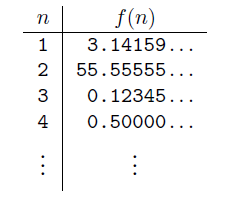
\includegraphics{img_3_7__0}
\end{figure}

\paragraph{}
Nous construisons le $x$ désiré en lui donnant sa représentation décimale. Notre objectif est de nous assurer que $x \neq f(n)$ pour n'importe quel $n$. Pour nous assurer que $x \neq f(1)$, nous changeons le premier chiffre de $x$ à n'importe quelle autre valeur différente de la première décimale de $f(1) = 3.\underline{\text{\textbf{1}}}4...$. Arbitrairement, mettons la première décimale de $x$ à 4. Pour nous assurer que $x \neq f(2)$, nous changeons le deuxième chiffre de $x$ par n'importe quelle valeur autre que le second chiffre décimal de $f(2) = 55.5\text{\underline{\textbf{5}}}5...$. Arbitrairement, mettons le à 6. Le troisième chiffre de $f(3)$ est $3$, donc nous modifions la troisième décimale de $x$ pour qu'elle soit différente de celle de $f(3)$, disons 4. 
\paragraph{}
Et ainsi de suite, en continuant ainsi à travers la diagonale du tableau, nous obtenons un $x$ qui est différent de tous les autres. Il est différent du premier car la première décimale de $x$ diffère de celle de $f(1)$, il est différent du deuxième car la deuxième décimale de $x$ diffère de celle de $f(2)$, etc. Comme montré dans le tableau ci-dessous, $x$ est différent de tous les autres. 

\begin{figure}[H]
   \centering
   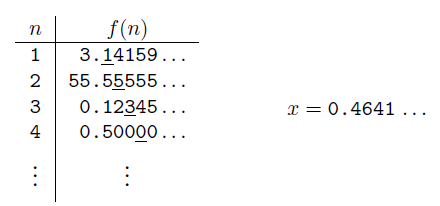
\includegraphics{img_3_7__1}
\end{figure}

\paragraph{}
Ce théorème a une application importante dans la théorie de la computation. Il montre que certains langages ne sont pas décidables voire même Turing-reconnaissables pour la simple raison qu'il y un nombre incomptable de langages alors qu'il n'y a qu'un nombre comptable de machines de Turing.
\paragraph{}
Parce qu'une machine de Turing ne peut reconnaître qu'un seul langage et qu'il y a davantage de langages que de TM, certains langages ne sont pas reconnu par n'importe quelle machine de Turing ! De tels langages ne sont pas Turing-reconnaissables.

\subsection{ Using a diagonalization argument, prove that some languages are not Turing-recognizable. }
Nous allons construire un tableau/matrice $A$ tel que, nous avons en ligne ($M_i$) : les machines de Turing et en colonne ($w_j$) : l'ensemble des mots des langages des machines de Turing $M_i$. La valeur en $A_{ij}$ vaut 1 si le mot est reconnu par la machine ($w_i \in L(M_i)$), sinon 0.
\begin{center}
\begin{tabular}{| c | c | c | c | c | c | c | c | c | c |}
	\hline
          & $w_0$ & $w_1$ & $w_2$ & $w_3$ & $w_4$ & ... & $w_j$ \\
    \hline
    $M_0$ & 0     & 1     & 1     & 1     & 1     & ... & 1     \\
    \hline
    $M_1$ & 0     & 0     & 1     & 0     & 1     & ... & 0     \\
    \hline
    $M_2$ & 1     & 0     & 1     & 1     & 0     & ... & 0     \\
    \hline
    $M_3$ & 1	  & 0     & 0     & 0     & 0     & ... & 1     \\
    \hline
    $M_4$ & 0     & 1     & 1     & 1     & 1     & ... & 0     \\
    \hline
    $...$ & ...   & ...   & ...   & ...   & ...   & ... & ...   \\
    \hline
    $M_i$ & 1     & 1     & 1     & ...   & 0     & 0   & 1     \\
\end{tabular}
\end{center}

Maintenant nous considérons un nouvel l'ensemble $T$ constitué des mots de la diagonale tel que :
\begin{itemize}
\item $w_j \in T$ si $w_j \not\in L(M_i)$ 
\item $w_j \not\in T$ si $w_j \in L(M_i)$ 
\end{itemize}
Alors nous avons obtenu un langage qui n'est reconnu par aucune machine de Turing \textbf{(CQFD)}.

\begin{center}
\begin{tabular}{| c | c | c | c | c | c | c | c | c | c |}
	\hline
          & $w_0$ & $w_1$ & $w_2$ & $w_3$ & $w_4$ & ... & $w_j$ \\
    \hline
    $M_0$ & \textcolor{red}{$\not{0}$ 1}     & 1     & 1     & 1     & 1     & ... & 1     \\
    \hline
    $M_1$ & 0     & \textcolor{red}{$\not{0}$ 1}     & 1     & 0     & 1     & ... & 0     \\
    \hline
    $M_2$ & 1     & 0     & \textcolor{red}{$\not{1}$ 0}     & 1     & 0     & ... & 0     \\
    \hline
    $M_3$ & 1	  & 0     & 0     & \textcolor{red}{$\not{0}$ 1}     & 0     & ... & 1     \\
    \hline
    $M_4$ & 0     & 1     & 1     & 1     & \textcolor{red}{$\not{1}$ 0}     & ... & 0     \\
    \hline
    $...$ & ...   & ...   & ...   & ...   & ...   & ... & ...   \\
    \hline
    $M_i$ & 1     & 1     & 1     & ...   & 0     & 0   & \textcolor{red}{$\not{1}$ 0}     \\
\end{tabular}
\end{center}


\subsection{ Prove that if a language A and its complement A are both Turing-recognizable, then A is Turing-decidable. }
\paragraph{Théorème} Un langage $A$ est décidable si et seulement si $A$ et son complémentaire sont Turing-reconnaissables. Autrement dit, un langage est decidable seulement lorsque celui-ci et sont complémentaires sont tous les deux Turing-reconnaissables.

\paragraph{Preuve} Nous avons deux choses à prouver. Premièrement, si $A$ est décidable, nous pouvons aisément voir que $A$ et sont complémentaire sont Turing-reconnaissables.N'importe quel langage décidable est Turing-reconnaissable, et le complément d'un décidable est aussi décidable. Deuxièmement, si $A$ et $\bar{A}$ sont Turing-reconnaissables, nous créons $M_{1}$ un reconnaisseur pour $A$ et $M_{2}$, un reconnaisseur pour $\bar{A}$.  La machine de Turing $M$ suivante est un décideur pour $A$: 
\paragraph{}
$M = $ "Sur l'input $w$ :
\begin{enumerate}
\item Exécuter $M_{1}$ et $M_{2}$ en parallèle sur l'input $w$.
\item Si $M_{1}$ accepte, on $accepte$ ; si $M_{2}$ accepte, on $rejette$."
\end{enumerate}
\paragraph{}
Exécuter les deux machines en parallèle signifie que $M$ possède deux rubans, une pour simuler $M_{1}$ et l'autre pour simuler $M_{2}$. Dans ce cas, M tourne en simulant une étape de chaque machine, et ça se poursuit jusqu'à ce que l'un d'eux \textit{accepte}. 
\paragraph{}
Maintenant, nous montrons que $M$ décide $A$. Chaque chaine de caractères $w$ est soit dans A, soit dans $\bar{A}$. Du coup, $M_{1}$ ou $M_{2}$ \textit{doit} accepter $w$. Parce que $M$ s'arrêtant chaque fois que $A$ ou $\bar{A}$ accepte, $M$ s'arrête donc toujours et donc est un décideur.
\paragraph{}
De plus, $M$ accepte toutes les chaines de caractères de $A$ et rejette toutes celles qui ne sont pas dans $A$. Donc, $M$ est un décideur pour $A$, et $A$ est décidable !

\subsection{Let A be a Turing-recognizable language consisting of descriptions of deciders. Prove that there exists a decidable language that is not decided by any decider described in A. (Exercise 4.28) }

\paragraph{} 
La solution se fait en deux étapes. Tout d'abord, nous construisons un nouveau langage, notons-le $Q$ qui ne sera décidé par aucune des machines de Turing $M_{i}$ en utilisant la technique de la diagonalisation. Ensuite, nous montrons comment construire un décideur pour $Q$ en utilisant le fait que $A$ est Turing-reconnaissable.

\paragraph{}
Le tableau suivant montre une diagonalisation similaire à celles qu'on a vu en cours.

\begin{figure}[H]
   \centering
   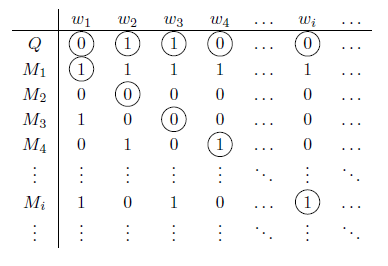
\includegraphics{img_3_10__0}
\end{figure}

\paragraph{}
Nous construisons donc un nouveau langage $Q$ qui ne correspond à aucun langage décidé par un décideur $M_{i}$, c'est-à-dire $Q$ ne correspond à aucun $L(M_{i})$ sur $w_{i}$. Formellement : $w_{i} \in Q ssi \not\in L(M_{i})$

\paragraph{}
Ainsi, aucune des $M_{i}$ ne décide $Q$.
Nous supposons, sans perte de généralité, que l'ordre des $w_{i}$ est dans l'ordre standard, c'est-à-dire ordonné par taille, puis de manière lexicographique. (a avant b, b avant c, etc.) Pour un alphabet fini donné $\Sigma$, il y a un nombre fini de nombre de taille finie, du coup il y a un algorithme $W$ qui énumère tous les mots de $\Sigma^{*}$ dans l'ordre lexicographique. 

\paragraph{}
Sachant que $A$ est Turing-reconnaissable, il existe un énumérateur pour $A$, comme démontré dans une autre question. Pour prouver que $Q$ est décidable, nous construisons la machine de Turing $D$ suivante :

\paragraph{}

$D = $ "sur l'entrée $w_{i}$ :
\begin{enumerate}
\item Déterminer la valeur de $i$ en utilisant l'énumérateur $W$, c'est-à-dire qu'on énumère tous les mots dans l'ordre standard tout en maintenant un compteur du nombre de mots énumérés et on stop dès qu'on rencontre $w_{i}$.

\item Énumerer les $M_{k}$ de $A$ en utilisant un énumérateur pour $A$. Stopper dès que nous avons énuméré $i$ décideurs différents, c'est-à-dire que le dernier décideur terminé par l'énumérateur est $M_{i}$.
\item Simuler $M_{i}$ sur $w_{i}$. Si $M_{i}$ accepte, on $rejette$. Si $M_{i}$ rejette, on $accepte$.
\end{enumerate}
\paragraph{}
$D$ est un décideur sachant que :
\begin{enumerate}
\item L'étape 1 et 2 exécutent un nombre fini d'étapes puisque $i$ est fini.
\item L'étape 3 s'arrête après un nombre fini d'étapes puisque $M_{i}$ est un décideur.
\end{enumerate}
\paragraph{}
$D$ accepte $w_{i}$ ssi $M_{i}$ rejette $w_{i}$. Sachant que $D$ et $M_{i}$ sont des décideurs, cela équivaut à dire que $w_{i} \in L(D)$ ssi $w_{i} \not\in L(M_{i})$, du coup $L(D) = Q$. $D$ est donc un décideur pour $Q$ et doooooonc $Q$ est décidable ! 


\subsection{Define the Halting Problem \texorpdfstring{$A_{TM}$}{Lg} and prove it is undecidable.}
\paragraph{}
Le problème de l'arrêt ou ($A_{TM}$) est un problème qui consiste à déterminer, à partir d'une description d'un programme et de son input, si le dit programme finira par s'arrêter ou pas. Alan Turing a prouvé qu'un algorithme permettant de résoudre le problème de l'arrêt pour toutes les paires $<$Programme - son Input$>$ \textbf{ne peut pas} exister. Il s'agit d'un problème indécidable pour les machines de Turing.

\paragraph{}
Il est à noter que $A_{TM}$ est \textit{Turing-reconnaissable (Turing recognizable)}. Donc, le théorème ci-dessus nous montre que les \textit{reconnaisseur (recognizers)} sont plus puissant que les décideurs. Exiger qu'une machine de Turing ait la capacité de s'arrête sur toutes les input va restreindre les différentes sortes de langage que la machine peut reconnaître. Mettons qu'on possède une machine de Turing $U$ qui reconnaisse $A_{TM}$. Cette machine devra donc s'exécuter comme suit: 
\paragraph{}
$U = $ "Sur l'input $<M, w>$, où $M$ est une machine de Turing et $w$ est une chaine de caractère: 
\begin{enumerate}
\item Simuler $M$ sur l'entrée $w$.
\item Si jamais $M$ entre dans son état d'acceptance, $U$ accepte; si jamais $M$ entre dans son état de rejet, $U$ rejette."
\end{enumerate}
\paragraph{}
À noter également que $U$ va boucler éternellement sur l'input $<M, w>$ si jamais $M$ boucle sur son input $w$. C'est donc pourquoi $U$ ne décide pas $A_{TM}$. Cette machine est appelée "machine de Turing universelle" (initialement proposée par Alan Turing). Elle est appelée "universelle" parce qu'elle peut simuler n'importe quelle autre machine de Turing à partir de la description de celle-ci. La machine de Turing universelle a joué un rôle important dans les débuts du développement des \textit{Ordinateur à programme enregistré}
\footnote{Un ordinateur à programme enregistré (ou calculateur à programme enregistré; en anglais stored-program computer) est un ordinateur qui enregistre les instructions des programmes qu'il exécute dans sa mémoire vive.
Un ordinateur avec une architecture de von Neumann enregistre ses données et ses instructions dans la même mémoire; un ordinateur avec une architecture Harvard enregistre ses données et ses instructions dans des mémoires séparées}.

\paragraph{} Mais tout ceci n'est qu'anecdotique et ne répond pas à la deuxième partie de la question qui est de prouver l'indécidabilité d'$A_{TM}$.

\paragraph{Théorème : $A_{TM}$ est indécidable}
\paragraph{Preuve que $A_{TM}$ est un problème indécidable} 
Définissons d'abord formellement $A_{TM}$ : 
\begin{equation}
A_{TM} = \{ <M, w> | M \text{ est une machine de Turing et } M \text{ accepte } w \}
\end{equation}
\paragraph{}
signifie que $A_{TM}$ correspond à l'ensemble des machines de Turing qui acceptent leur entrée.
\paragraph{}
Nous supposons que $A_{TM}$ soit décidable et obtenons une contradiction. Donc, on créé une machine de Turing $H$ qui est un décideur pour $A_{TM}$. Sur l'entrée $<M, w>$, où $M$ est une machine de Turing et $w$ est une chaine de caractère, $H$ s'arrêtera et acceptera si jamais $M$ accepte $w$. De plus, $H$ s'arrêtera également et rejettera si jamais $M$ rejette $w$. En d'autres termes, nous supposons que $H$ est une machine de Turing où : 

\begin{equation}
H(<M, w>) = \left\{
              \begin{array}{ll}
                  accepte \text{ si } M \text{ accepte } w \\
                  refuse  \text{ si } M \text{ refuse }  w
              \end{array}
            \right.
\end{equation}

\paragraph{}
Maintenant, construisons encore une nouvelle machine de Turing $D$ avec $H$ comme sous-routine. Cette nouvelle machine de Turing appellera $H$ pour déterminer ce que $M$ fait lorsque l'entrée de $M$ est sa propre description $<M>$. Une fois que $D$ a déterminé cette information, elle fait l'opposé. C'est-à-dire que $D$ rejettera si $M$ accepte et acceptera si $M$ rejette.

Voici la description de $D$ :
\paragraph{}
$D = $ "Sur l'entrée $<M>$, où $M$ est une machine de Turing :
\begin{enumerate}
\item Exécuter $H$ sur l'entrée $<M, <M>>$.
\item Faire l'opposé de ce que $H$ fait. C'est-à-dire, si $H$ accepte, $rejetter$; et si $H$ rejette, $accepter$."
\end{enumerate}

\paragraph{}
Il ne faut pas être confus par la notion d'exécuter une machine avec sa propre description comme entrée. C'est similaire à exécuter un programme avec lui-même comme entrée, chose qui arrive parfois en pratique. Par exemple, un compilateur est un programme qui traduit d'autres programmes. Un compilateur pour le langage \textit{Python} peut lui-même être écrit en Python, donc exécuter un programme sur lui-même peut avoir du sens.

\paragraph{}
En résumé, $D(<M>)$ accepte si $M$ rejette $M$, et rejette si $M$ accepte $<M>$. Que se passe-t-il lorsque nous exécutons $D$ avec sa propre description $<D>$ en input ? Dans ce cas, nous avons que $D(<D>)$ \textit{accepte} si $D$ rejette $<D>$ et \textit{rejette} si $D$ accepte $<D>$. Peu importe ce que fait $D$, la machine est obligé de retourner l'opposé, ce qui est contradictoire. Du coup, ni $H$, ni $D$ ne peuvent exister. CQMD (Ce que Mourad démontre lol.)

\paragraph{}
Résumons les étapes de cette preuve. Premièrement, nous supposons une machine de Turing $H$ qui décide $A_{TM}$. Nous utilisons $H$ pour construire une autre machine de Turing $D$ qui prend une description de machine $<M>$ en input. Finalement, nous exécutons $D$ avec sa propre description $<D>$ en input. La machine fera les actions suivantes, avec la dernière ligne qui est une contradiction :
\begin{itemize}
\item $H$ accepte $<M, w>$ exactement lorsque $M$ accepte $w$.
\item $D$ rejette $<M>$ exactement lorsque $M$ accepte $<M>$.
\item $D$ rejette $<D>$ exactement lorsque $D$ accepte $<D>$.
\end{itemize}


\subsection{Define the Post Correspondence Problem and prove it is undecidable. }
Le problème de post-correspondance consiste, à partir d'un ensemble $n$ dominos,à déterminer s'il existe une suite de dominos (avec répétitions) telle que les caractères du haut sont les même que les caractères du bas.
\paragraph{}
\textbf{Exemple :}
\[\{[\frac{b}{ca}], [\frac{a}{ab}], [\frac{ca}{a}], [\frac{abc}{c}]\}\]
Une correspondance existe et est donnée par la suite suivante :
\[\{ [\frac{a}{ab}], [\frac{b}{ca}], [\frac{ca}{a}], [\frac{a}{ab}], [\frac{abc}{c}] \}\]

\paragraph{}
Une instance de PCP est une collection $P$ de dominos :
\[\{ [\frac{t_1}{b_1}], [\frac{t_2}{b_2}], [\frac{t_3}{b_3}], ..., [\frac{t_k}{b_k}] \}\]
Une correspondance est une séquence de $i_1, i_2, i_3, ..., i_i$ tel que $t_1, t_2,..., t_k = b_1, b_2, ..., b_k$
Le problème est de savoir déterminer si l'ensemble P possède une correspondance. Définissons PCP = \(\{ (P) | P$ est une instance positive du problème de post-correspondance$ \}\)

\paragraph{}
\textbf{Theoreme : PCP est indécidable}
\paragraph{}
\textbf{Preuve}
\paragraph{}
Nous allons modifier légèrement le PCP en donnant la règle que la correspondance doit toujours commencer avec le premier domino $\frac{t_1}{b_1}$
\paragraph{}
Maintenant nous avons MPCP : \( \{ (P)|P$ est une instance positive du problème de post-correspondance qui commence avec le premier domino.$ \} \)

Nous avons une TM $R$ qui décide de PCP et construit $S$ qui décide $A_{TM}$.

\paragraph{}
Dans ce cas, S construit une instance positive de PCP ssi $M$ accepte $w$. Pour cela, S construit dans un premier temps, une instance P' de MPCP. Nous allons décrire cette création en 7 étapes. Chacun d'eux réalise un aspect particulier de la simulation de $M$ sur $w$.

\begin{enumerate}
\item Le premier domino corresponds à la premiere configuration de $M$ sur $w$ tel que :
	\[ [\frac{t_1}{b_1}] => [\frac{\#}{\#q_0w_1w_2...w_n\#}] \] 
    Nous ajoutons donc le domino dans P'.
    \paragraph{}
    Nous avions défini la règle, pour MPCP, que la correspondance doit toujours commencer avec le premier domino. La partie basse du domino correspond à la configuration de départ (de l'éxecution positive de $M$ sur $w$) et la partie haute contient la configuration précédente (dans ce cas-ci = \#). 
    
    \item \(\forall a, b \in \Gamma\) et \(\forall q,r \in Q\) où q n'est pas $q_{reject}$
    \paragraph{}
    Si $\delta(q,a)$ =  (r,b,R) : ajoutez $[\frac{qa}{br}]$ dans P'.
    
    \item $\forall a,b,c \in \Gamma$ et $\forall q,r \in Q$ où q n'est pas $q_{reject}$
    \paragraph{}
    Si $\delta(q,a)$ = (r,b,L) : ajoutez $[\frac{cqa}{rcb}]$ dans P'.
    
    \item $\forall a \in \Gamma$ : ajoutez $[\frac{a}{a}]$ dans P'.
    \paragraph{}
    \textbf{Exemple de ce que nous avons fait pour l'instant :}
    \paragraph{}
    Prenons comme cas que $\Gamma = \{0, 1, 2, \textvisiblespace \}$, que $w$ est la string "0100" et que l'etat initial de $M$ est $q_0$. 
    \paragraph{}
    Part 1 : Ajoutez le premier domino dans P' : $[\frac{\#}{\#q_00100\#}]$
    \paragraph{}
    Part 2 : Nous avons à l'état $q_0$, lorsqu'il lis un $0$, fait appel à une fonction de transition qui va dire à $M$ de passer à l'état $q_7$, d'écrire 2 et de bouger la tête vers la droite : $\delta(q_0,0) = (q_7, 2,R)$ donc le domino : $\frac{q_00}{2q_7}$. Nous avons dans P' maintenant : 
    \[ [\frac{\#}{\#q_00100\#}], [\frac{q_00}{2q_7}]\]
    \paragraph{}
    Part 4 : On complète P' par un ou plusieurs domino(s) suivant(s) afin de respecter l'égalité entre la partie haute et basse :
    	\[ [\frac{0}{0}], [\frac{1}{1}], [\frac{2}{2}], [\frac{\textvisiblespace }{\textvisiblespace }]\]
        Nous obtenons donc dans P' :
        \begin{figure}[H]
        	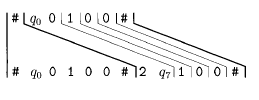
\includegraphics[]{img_3_12__0}
        \end{figure}
        \paragraph{}
        Note : Le domino $[\frac{\#}{\#}]$ est ajouté grâce à la part 5 (que nous allons voir).
        
        \item Ajoutez $[\frac{\#}{\#}]$ et $[\frac{\#}{\textvisiblespace \#}]$ dans P'.
        \paragraph{}
        Le premier domino nous permet de copier le symbole $\#$ qui marque la fin d'une configuration. Le second permet de rajouter l'espace vide à la fin d'une configuration pour simuler les infinies espaces vide de droite qui ont été supprimé quand nous avons ecrit la configuration.
        
        \item $\forall a \in \Gamma$, ajoutez $[\frac{aq_{accept}}{q_{accept}}]$ et $[\frac{q_{accept}a}{q_{accept}}]$ dans P'
        
        \item Finalement, nous ajoutons le domino qui complète la correspondance : \[[\frac{q_{accept\#\#}}{\#}]\]
\end{enumerate}

Nous savons comment construire P', qui est une instance positive de MPCP. Maintenant nous allons convertir P' en P, qui est une instance positive de PCP. L'idée est de construire le besoin de toujours commencer par le premier domino et de ne plus le dire explicitement (The idea is to build the requirement of starting with the first domino directly into the problem so that stating the explicit requirement becomes unnecessary). Nous allons introduire quelques notions :
\begin{itemize}
\item $\star u = \star u_1 \star u_2 \star u_3 \star ... \star u_n$
\item $u \star = u_1 \star u2 \star u_3 \star ... \star u_n \star$
\item $ \star u \star = \star u_1 \star u_2 \star u_3  \star ... \star u_n \star$
\end{itemize}
\paragraph{}
Ici, nous avons $\star u$ où nous ajoutons $\star$ avant chaque caractère de u, $u \star$ après chaque caractere de u et $\star u \star$
avant et après chaque caractere de u. Pour convertir P' en P, une instance de PCP, nous allons faire comme ceci : Si P' est une collection : 
\[ [\frac{t_1}{b_1}], [\frac{t_2}{b_2}], [\frac{t_3}{b_3}], ..., [\frac{t_k}{b_k}] \]
Alors nous avons pour P :
\[ [\frac{\star t_1}{\star b_1 \star }], [\frac{\star t_1}{b_1 \star }], [\frac{\star t_2}{b_2 \star }], [\frac{\star t_3}{b_3 \star }], ..., [\frac{\star t_k}{b_k \star }], [\frac{\star \Diamond}{\Diamond}] \]

Considérons P comme une instance de PCP, nous voyons que nous pouvons commencer qu'avec le premier domino : $[\frac{\star t_1}{\star b_1 \star }]$. Parce que c'est le seul qui commence avec le même symbole dans la partie haute et basse : $\star$. En forçant la correspondance à commencer avec le premier domino , nous ne devons plus demander explicitement à S.(ça se fera automatiquement) 
\paragraph{}
\textbf{CQFD}

\subsection{State Rice’s Theorem and prove it. Give two problems that can be proved undecidable by applying Rice’s Theorem. }

\paragraph{} Informellement, le théorème de Rice dit que le problème consistant à déterminer si une machine de Turing possède telle propritété non-triviale est un problème indécidable.

\paragraph{Réponse de Gabriel Ortega}
\paragraph{Théorème} Formellement, soit $P$ le langage consistant en la description de plusieurs machines de Turing où $P$ remplit deux conditions :
\begin{enumerate}
  \item $P$ est une propriété qui n'est pas trivial. $P$ contient certaines mais pas toutes les descriptions d'une machine de Turing.
  \item $P$ fait parti des propriétés du langage de la machine de Turing (lorsque $L(M_{1}) = L(M_{2})$, nous avons que la description de la machine de Turing $<M_{1}> \in P$ ssi $<M_{2} \in P$
\end{enumerate}


\paragraph{Preuve} Supposons que $P$ (par amour de la contradiction $\varheart$) soit un langage décidable satisfaisant les propriétés et $R_{P}$ une machine de Turing qui décide $P$.

\paragraph{}
Nous montrons comment décider $A_{TM}$ en utilisant $R_{P}$ en construisant une machine de Turing $S$.Tout d'abord, posons $T_{\emptyset}$ une TM qui rejette toujours. Donc, $L(T_{\emptyset}) = \emptyset$ \textit{(Aucun langage n'est accepté par $T_{\emptyset}$)}. Il est permis de supposer que $<T_{\emptyset}> \not\in P$ parce qu'il est possible de procéder avec $\overline{P}$ au lieu de $P$ si $<T_{\emptyset}> \in P$ 

\paragraph{}
Parce que $P$ n'est pas trivial, il existe une machine de Turing $T$ avec $<P> \in P$. On conçoit $S$ pour décider d'$A_{TM}$ en utilisant la capacité de $R_{P}$ à distinguer $T$ de $T_{\emptyset}$.

\paragraph{}
$S$ = "Sur l'entrée $<M, w>$ :
\begin{enumerate}
\item Utiliser $M$ et $w$ pour construire la machine de Turing $M_{w}$ suivante : \\
$M_{w} = "$ sur l'entrée $x$:
	\begin{enumerate}[I]
	\item Simuler $M$ sur $w$. Si $M$ s'arrête et rejette, \textit{on rejette}. Sinon, étape II.
    \item Simuler $T$ sur $x$. Si $T$ accepte, \textit{accepter}."
	\end{enumerate}
\item Utiliser la mmachine de Turing $R_{P}$ pour déterminer si $<M_{w}> \in P$. Si oui, \textit{on accepte} ; Sinon,  \textit{on rejette}.
\end{enumerate}
\paragraph{}
La machine de Turing $M_{w}$ simule $T$ si $M$ accepte $w$. Ainsi $L(M_{w}) = L(T)$ si $M$ accepte $w$ ; sinon  $L(M_{w}) = \emptyset$. Conclusion, $<M_{w}> \in P$ ssi $M$ accepte $w$.


\paragraph{Exemple 1}
Soit $T = \{<M> | \text{ $M$ est une machine de Turing qui accepte } w^{R} \text{ lorsqu'elle accepte } w\}$, 
où $w = w_{1}w_{2}w_{3}...w_{n}$ et $w^{R} = w_{n}w_{n-1}...w_{1}$. (L'inverse de $w$ en somme)
\paragraph{T est indécidable}
\paragraph{Preuve} (Par le théorème de Rice) Soit $P$ une propriété non-triviale tel que $P = \{A | w \in A \Leftrightarrow w^{R} \in A \}$ \textit{(P est défini comme l'ensemble des langages où chaque mot de $A$ possède son inverse dans $A$ également.)}. Nous devons montrer que $P$ est une propriété non triviale.

\paragraph{}
Par exemple, $\{01\} \not\in P$, donc $P \neq \mathcal{P}(\Sigma^{*})$ ; et $\{1\} \in P$ donc $P \neq \emptyset$.

\paragraph{Exemple 2}
lol
\subsection{Give an example of a language that is not Turing-recognizable. }
\paragraph{Réponse de Gabriel Ortega}
\paragraph{}
$\overline{A_{TM}}$ n'est pas un langage Turing-reconaissable.

\paragraph{Preuve} Nous savons que $A_{TM}$ est Turing-reconnaissable. Si $\overline{A_{TM}}$ était également Turing-reconnaissable, alors $A_{TM}$ serait décidable, ce qui n'est pas le cas. 
\paragraph{}
Ainsi, $\overline{A_{TM}}$ n'est pas Turing-reconnaissable.




\subsection{Describe the 3x + 1 problem (also known as Collatz problem/conjecture), and show that if Ai were decidable, then there exists a Turing machine guaranteed to state the answer to the 3x + 1 problem (Exercise 5.31).}
\paragraph{Pas vu en cours, à ne pas connaître ! YEAH}

\section{Time Complexity}

\subsection{Prove that for t(n)$\geq$n, every t(n)-time nondeterministic Turing machine has an equivalent
$2^{O(t(n))}$-time deterministic Turing machine.}
\paragraph{Théorème } Soit $t(n)$ une fonction où $t(n) \geq n$. Alors, toutes les machines de Turing non-déterministes mono-ruban s'exécutant en un temps de l'ordre de $t(n)$ possèdent un équivalent déterministe s'exécutant en $2^{O(t(n))}$.

\paragraph{Preuve} Soit $N$ une machine de Turing non-déterministe s'exécutant en un temps $t(n)$. Nous construisons une machine de Turing déterministe $D$ qui simule $N$ comme montré dans un théorème plus haut en cherchant dans l'arbre d'exécution non-déterministe de $N$. Maintenant, analysons cette simulation. Sur une entrée de taille $n$, chaque branche de l'exécution non-déterministe de $N$ possède une longueur d'au plus $t(n)$. Chaque noeud dans l'arbre peut avoir $b$ enfants, où $b$ est le nombre maximum de choix possibles en fonction de la fonction de transition de $N$.
\paragraph{}
Du coup, le nombre total de feuilles dans l'arbre est d'au plus $b^{t(n)}$. La simulation procède en explorant l'arbre par niveau de profondeur. Donc, elle visite tous les noeuds d'une profondeur $d$ avant de passer à la profondeur $d+1$. 
\paragraph{}
Le nombre total de noeuds dans l'arbre est inférieur au double du nombre de feuilles, donc nou pouvons borner cette valeur par $O(b^{t(n)})$. Le temps pris pour aller de la racine vers un noeud est de $O(t(n))$. Donc, le temps d'exécution de $D$ est $O(t(n) * b^{t(n)}) = 2^{O(t(n))}$

Aussi, comme décrit dans le théorème plus haut, la machine de Turing $D$ possède trois rubans. Convertir ça en un mono-ruban prend un temps quadratique par rapport au temps d'exécution normal (par le théorème 7.8 du livre de référence). Ainsi, le temps d'exécution mono-ruban est $(2^{O(t(n))})^{2} = 2^{O(2t(n))} = 2^{O(t(n))}$. CQFD.

\subsection{Give two definitions of the complexity class NP and prove that they are equivalent.}
\begin{itemize}
\item NP est la classe des langages qui possèdent un vérificateur en temps polynomial.
\item NP est la classe des langages \textit{décidés} en temps polynomial par une machine de Turing non-déterministe. $(NP = \bigcup_{k} NTIME(n^{k}))$
\end{itemize}

\subsection{Explain why all problems in NP can be decided in time $2^{O(n^{k})}$ for some k.}
lol

\subsection{Is it the case that P $\subseteq$ NP? Is it the case that NP $\subseteq$ P? Explain.}
lol

\subsection{Define the notion of polynomial time (mapping) reduction and show that if A is polynomial time reducible to B and B $\in$ P, then A $\in$ P.}
lol

\subsection{Define the notion of NP-completeness.}
\paragraph{}
Un langage B est \textit{NP-complet} s'il satisfait deux conditions :
\begin{enumerate}
  \item B est dans NP
  \item tous les langages A dans NP peuvent se réduire en temps polynomial à B.
\end{enumerate}

\subsection{Prove the following two statements:}
	\begin{itemize}
		\item \textbf{If B is NP-complete and B $\in$ P then P = NP.}
		\item \textbf{If B is NP-complete and B $\leq_{p}$ C and C $\in$ NP then C is NP-complete.}
	\end{itemize}
lol

\subsection{State the Cook-Levin Theorem and give a detailed outline of the proof.}
lol

\subsection{Define the 3-SAT problem and prove it is NP-complete.}
lol

\subsection{Define the VERTEX-COVER problem and prove it is NP-complete.}
lol

\subsection{Define the HAMILTONIAN-PATH problem and prove it is NP-complete.}
lol

\subsection{Define the CLIQUE problem and prove it is NP-complete.}
lol

\subsection{Define the INDEPENDENT-SET problem and prove it is NP-complete. (Exercise)}
lol

\subsection{Define the 3-COLORING problem and prove it is NP-complete. (Exercise 7.27)}
lol

\subsection{Define the SUBSET-SUM problem and prove it is NP-complete.}
lol

\subsection{Give a dynamic programming algorithm for the SUBSET-SUM problem and explain why it does not imply P = NP.}
lol

\subsection{Show that if $P = NP$, you can determine a satisfying assignment to a $3-CNF$ formula in polynomial time, if one exists (Exercise 7.36).}
lol

\subsection{Show that if $P = NP$ you can determine a maximum-size clique in a graph in polynomial time (Exercise 7.38, see solution in the textbook).}
If you assume that P = NP, then CLIQUE $\in$ P, and you can test whether G contains a clique of size k in polynomial time, for any value of k. By testing whether G contains a clique of each size, from 1 to the number of nodes in G, you can determine the size t of a maximum clique in G in polynomial time. Once you know t, you can find a clique with t nodes as follows. For each node x of G, remove x and calculate the resulting maximum clique size. If the resulting size decreases, replace x and continue with the next node. If the resulting size is still t, keep r permanently removed and continue with the next node. When you have considered all nodes in this way, the remaining nodes are a t-clique.

\section{Space Complexity}

\subsection{Define the space complexity of deterministic and nondeterministic Turing machines, and give an example of a problem that can be solved in O(t(n)) space, but for which we do not know any O(t(n))-time algorithm, for some function t(n).}
lol

\subsection{State and prove Savitch's Theorem, and show it implies PSPACE = NPSPACE.}
\paragraph{}
Le théorème de Savitch stipule qu'une machine déterministe peut simuler une machinque de Turing non-déterministe en utilisant très peu d'espace.
En compléxité spatiale, le théorème de Savitch montre que n'importe quelle TM non-déterministe qui s'exécute en espace $f(n)$ peut être convertie en TM déterministe s'exécutant seulement en espace $f^{2}(n)$.

\paragraph{Théorème} 
Pour n'importe quelle fonction $f : \mathbb{N} \rightarrow \mathbb{R}^{+}$, où $f(n) \geq n$, $NSPACE(f(n)) \subseteq SPACE(f^{2}(n))$.
\paragraph{Idée de preuve} Considérons une approche un peu spéciale. Soit deux configurations $c1$ et $c2$ d'une NTM, et un nombre $t$. Nous testons si peut aller de $c1$ à $c2$ en $t$ étapes en utilisant seulement $f(n)$ espace. Ce problème s'appelle \textit{the yieldability problem} (le problème du rendement ?). En résolvant ce problème, où $c1$ est la configuration de départ, $c2$ est la configuration d'acceptance, et $t$ est le nombre maximum d'étapes que la NTM peut utiliser, nous pouvons déterminer si la machine accepte son input.

\paragraph{}
Nous donnons un algorithme déterministe récursif qui résout ce problème. Il opère en cherchant une configuration intermédiaire $c_{m}$, et teste récursivement, si :
\begin{enumerate}
\item $c1$ peut aller vers $c_{m}$ en $\frac{t}{2}$ étapes, et
\item si $c_{m}$ peut aller vers $c2$ en $\frac{t}{2}$ étapes.
\end{enumerate}

\paragraph{}
Réutiliser l'espace pour chacun des deux tests récursifs permet des économies d'espace significatives. Aussi, cet algorithme a besoin d'espace pour stocker la pile de récursivité. Chaque niveau de la récursivité utilise $O(f(n))$ espace pour stocker une configuration.

La profondeur de la récursion est $log(t)$, où $t$ est le temps maximum que la machine non déterministe peut utiliser sur n'importe quelle branche. Nous avons $t = 2^{O(f(n))}$, donc $log(t) = O(f(n))$. Du coup, la simulation déterministe utilise $O(f^{2}(n))$ espace.

\paragraph{Preuve} Soit $N$, une NTM décidant le langage $A$ en espace $f(n)$. Nous construisons une TM déterministe $M$ qui décide $A$. La machine $M$ utilise une procédure "$CANYIELD$", qui teste une des configurations de N peut en produire une autre dans un nombre spécifié d'étapes. Cette procédure résout le \textit{yieldability problem} décrit plus haut.

\paragraph{} 
Soit $w$, une chaine de caractère considéré comme l'input de $N$. Pour les configurations $c1$ et $c2$ de $N$, et un entier $t$, $CANYIELD(c1, c2, t)$ retourne $accepte$ si $N$ peut aller de la configuration $c1$ à $c2$ en $t$ (ou moins) étapes le long d'un chemin non-déterministe. Sinon, $CANYIELD$ retourn $rejette$. Pour plus de commodité, nous supposons que $t$ est une puissance de 2.
\paragraph{}
CANYIELD = “On input c1, c2, and t:
\begin{enumerate}
\item Si $t = 1$, alors tester directement si $c1 = c2$ ou si $c1$ produit $c2$ en une étape en accord avec la fonction de transition de $N$. $accepte$ si l'un des tests réussi, $rejette$ si les deux échouent.
\item Si $t > 1$, alors pour chaque configuration $c_{m}$ de $N$ utilisant $f(n)$ espace :
\item $| $ Exécuter $CANYIELD(c1, c_{m}, \frac{t}{2})$
\item $| $ Exécuter $CANYIELD(c_{m}, c2, t)$
\item $| $ Si l'étape 3 et 4 acceptent tous les deux, alors $accepter$
\item Si toujours pas d'$accepte$, alors $rejette$
\end{enumerate}
\paragraph{}
Maintenant, nou définissons $M$ pour simuler $N$ comme suit. Nous modifions tout d'abord $N$ pour que lorsqu'elle accepte, elle vide son ruban et bouge sa tête de lecture/écriture à la cellule la plus à gauche, entrant ainsi dans une configuration appelée $c_{accepte}$. Nous définissons $c_{start}$ la configuration de départ de $N$ sur l'entrée $w$. Nous choisissons une constante $d$ pour que $N$ ne puisse pas excéder $2^{d.f(n)}$ en utilisant un ruban de taille $f(n)$, où $n$ est la longueur de $w$. Nous savons ainsi que $2^{d.f(n)}$ représente une borne supérieure au temps d’exécution de n’importe quelle branche de $N$ sur $w$ :
\paragraph{}
$M$ = "Sur l'entrée $w$ :
\begin{enumerate}
\item Retourner le résultat de $CANYIELD(c_{accepte}, c_{start}, 2^{d.f(n)})$
\end{enumerate}
"\textit{
A chaque appel récursif de $CanYield$, cet algorithme conserve $c1$, $c2$ et $t$ sur le stack de manière à pouvoir restaurer ces valeurs au retour de l’appel récursif. Chaque niveau de récursion utilise donc un espace additionnel de mémoire qui s’exprime en $O(f(n))$. De plus, chaque niveau de récursion divise la valeur de $t$ par 2. Au départ, $t = 2^{d.f(n)}$ , donc la profondeur de la récursion s’exprime en $O(log (2^{d.f(n)}))$, c.-à-d en $O(f(n))$. Par conséquent, l’espace mémoire total requis s’exprime en $O(f^{2}(n))$.}" - François Santy
\paragraph{Implication de $PSPACE = NPSPACE$}
\begin{itemize}
\item PSPACE est la classe des langages qui sont décidables en espace polynomial sur une machine de Turing déterministe.
\item La classe NPSPACE est la classe des langages qui sont décidables en espace polynomial sur une machine de Turing non déterministe.
\end{itemize}
Grâce au théorème de Savitch, $PSPACE = NPSPACE$ puisque le carré de n’importe quel polynôme est encore un polynôme.
\subsection{Define the notion of PSPACE-completeness.}
\paragraph{}
Un langage $B$ est $PSPACE-COMPLET$ s'il satisfait deux conditions :
\begin{enumerate}
  \item $B$ est dans PSPACE
  \item Tous les langages A dans $PSPACE$ peuvent se réduire à $B$ en temps polynomial.
\end{enumerate}

\subsection{Define the TQBF problem and prove it is in PSPACE.}
lol

\subsection{Prove that TQBF is PSPACE-complete.}
lol

\subsection{Explain the interpretation of the TQBF problem as a game between an existential and a universal player.}
lol

\subsection{What do we know about the relations between the complexity classes P, NP, PSPACE, and EXPTIME? Explain}
lol

\end{document}
